\documentclass{article}\usepackage[]{graphicx}\usepackage[]{color}
% maxwidth is the original width if it is less than linewidth
% otherwise use linewidth (to make sure the graphics do not exceed the margin)
\makeatletter
\def\maxwidth{ %
  \ifdim\Gin@nat@width>\linewidth
    \linewidth
  \else
    \Gin@nat@width
  \fi
}
\makeatother

\definecolor{fgcolor}{rgb}{0.345, 0.345, 0.345}
\newcommand{\hlnum}[1]{\textcolor[rgb]{0.686,0.059,0.569}{#1}}%
\newcommand{\hlstr}[1]{\textcolor[rgb]{0.192,0.494,0.8}{#1}}%
\newcommand{\hlcom}[1]{\textcolor[rgb]{0.678,0.584,0.686}{\textit{#1}}}%
\newcommand{\hlopt}[1]{\textcolor[rgb]{0,0,0}{#1}}%
\newcommand{\hlstd}[1]{\textcolor[rgb]{0.345,0.345,0.345}{#1}}%
\newcommand{\hlkwa}[1]{\textcolor[rgb]{0.161,0.373,0.58}{\textbf{#1}}}%
\newcommand{\hlkwb}[1]{\textcolor[rgb]{0.69,0.353,0.396}{#1}}%
\newcommand{\hlkwc}[1]{\textcolor[rgb]{0.333,0.667,0.333}{#1}}%
\newcommand{\hlkwd}[1]{\textcolor[rgb]{0.737,0.353,0.396}{\textbf{#1}}}%
\let\hlipl\hlkwb

\usepackage{framed}
\makeatletter
\newenvironment{kframe}{%
 \def\at@end@of@kframe{}%
 \ifinner\ifhmode%
  \def\at@end@of@kframe{\end{minipage}}%
  \begin{minipage}{\columnwidth}%
 \fi\fi%
 \def\FrameCommand##1{\hskip\@totalleftmargin \hskip-\fboxsep
 \colorbox{shadecolor}{##1}\hskip-\fboxsep
     % There is no \\@totalrightmargin, so:
     \hskip-\linewidth \hskip-\@totalleftmargin \hskip\columnwidth}%
 \MakeFramed {\advance\hsize-\width
   \@totalleftmargin\z@ \linewidth\hsize
   \@setminipage}}%
 {\par\unskip\endMakeFramed%
 \at@end@of@kframe}
\makeatother

\definecolor{shadecolor}{rgb}{.97, .97, .97}
\definecolor{messagecolor}{rgb}{0, 0, 0}
\definecolor{warningcolor}{rgb}{1, 0, 1}
\definecolor{errorcolor}{rgb}{1, 0, 0}
\newenvironment{knitrout}{}{} % an empty environment to be redefined in TeX

\usepackage{alltt}
\usepackage[sc]{mathpazo}
\renewcommand{\sfdefault}{lmss}
\renewcommand{\ttdefault}{lmtt}
\usepackage[T1]{fontenc}
\usepackage{geometry}
\geometry{verbose,tmargin=2.5cm,bmargin=2.5cm,lmargin=2.5cm,rmargin=2.5cm}
\setcounter{secnumdepth}{2}
\setcounter{tocdepth}{2}
\usepackage[unicode=true,pdfusetitle,
 bookmarks=true,bookmarksnumbered=true,bookmarksopen=true,bookmarksopenlevel=2,
 breaklinks=false,pdfborder={0 0 1},backref=false,colorlinks=false]
 {hyperref}
\hypersetup{
 pdfstartview={XYZ null null 1}}

\makeatletter
%%%%%%%%%%%%%%%%%%%%%%%%%%%%%% User specified LaTeX commands.
\renewcommand{\textfraction}{0.05}
\renewcommand{\topfraction}{0.8}
\renewcommand{\bottomfraction}{0.8}
\renewcommand{\floatpagefraction}{0.75}

\makeatother
\IfFileExists{upquote.sty}{\usepackage{upquote}}{}
\begin{document}



\title{\title{}}



\maketitle
The results below are generated from an R script.

\begin{knitrout}
\definecolor{shadecolor}{rgb}{0.969, 0.969, 0.969}\color{fgcolor}\begin{kframe}
\begin{alltt}
\hlkwd{install.packages}\hlstd{(}\hlstr{"rattle"}\hlstd{)}
\end{alltt}
\begin{verbatim}
## Error in install.packages : Updating loaded packages
\end{verbatim}
\begin{alltt}
\hlkwd{library}\hlstd{(here)}
\hlkwd{library}\hlstd{(tidyverse)}
\hlkwd{library}\hlstd{(ggplot2)}
\hlkwd{library}\hlstd{(ggpubr)}
\hlkwd{library}\hlstd{(knitr)}
\hlkwd{library}\hlstd{(rpart)}
\hlkwd{library}\hlstd{(rpart.plot)}
\hlkwd{library}\hlstd{(rattle)}
\hlkwd{library}\hlstd{(RColorBrewer)}


\hlstd{mydata} \hlkwb{<-} \hlkwd{read.csv}\hlstd{(}\hlstr{"Final_Project_FlixGem.csv"}\hlstd{)}


\hlstd{mydata} \hlkwb{<-} \hlstd{mydata} \hlopt \hlkwd{select}\hlstd{(Title, Languages, Series.or.Movie, Hidden.Gem.Score, Runtime, Director, IMDb.Score, Rotten.Tomatoes.Score,}
                            \hlstd{Metacritic.Score, Release.Date, Summary)}


\hlstd{mydata} \hlkwb{<-} \hlstd{mydata} \hlopt \hlkwd{filter}\hlstd{(Series.or.Movie} \hlopt{==} \hlstr{'Movie'}\hlstd{)}

\hlstd{mydata} \hlkwb{<-} \hlkwd{na.omit}\hlstd{(mydata)}

\hlstd{testdata} \hlkwb{<-} \hlstd{mydata} \hlopt \hlkwd{mutate}\hlstd{(}\hlkwc{FirstLanguage} \hlstd{=} \hlkwd{sub}\hlstd{(}\hlstr{",.*"}\hlstd{,} \hlstr{""}\hlstd{, mydata}\hlopt{$}\hlstd{Languages))}

\hlkwd{view}\hlstd{(testdata)}


\hlstd{hyper_grid} \hlkwb{<-} \hlkwd{expand.grid}\hlstd{(}
  \hlkwc{minsplit} \hlstd{=} \hlkwd{seq}\hlstd{(}\hlnum{5}\hlstd{,} \hlnum{20}\hlstd{,} \hlnum{1}\hlstd{),}
  \hlkwc{maxdepth} \hlstd{=} \hlkwd{seq}\hlstd{(}\hlnum{8}\hlstd{,} \hlnum{15}\hlstd{,} \hlnum{1}\hlstd{)}
\hlstd{)}

\hlstd{models} \hlkwb{<-} \hlkwd{list}\hlstd{()}

\hlkwa{for} \hlstd{(i} \hlkwa{in} \hlnum{1}\hlopt{:}\hlkwd{nrow}\hlstd{(hyper_grid)) \{}

  \hlcom{# get minsplit, maxdepth values at row i}
  \hlstd{minsplit} \hlkwb{<-} \hlstd{hyper_grid}\hlopt{$}\hlstd{minsplit[i]}
  \hlstd{maxdepth} \hlkwb{<-} \hlstd{hyper_grid}\hlopt{$}\hlstd{maxdepth[i]}

  \hlcom{# train a model and store in the list}
  \hlstd{models[[i]]} \hlkwb{<-} \hlkwd{rpart}\hlstd{(}
    \hlkwc{formula} \hlstd{= Hidden.Gem.Score} \hlopt{~} \hlstd{Runtime} \hlopt{+} \hlstd{IMDb.Score} \hlopt{+} \hlstd{Rotten.Tomatoes.Score} \hlopt{+} \hlstd{Metacritic.Score} \hlopt{+} \hlstd{FirstLanguage,}
    \hlkwc{data}    \hlstd{= testdata,}
    \hlkwc{method}  \hlstd{=} \hlstr{"anova"}\hlstd{,}
    \hlkwc{control} \hlstd{=} \hlkwd{list}\hlstd{(}\hlkwc{minsplit} \hlstd{= minsplit,} \hlkwc{maxdepth} \hlstd{= maxdepth)}
  \hlstd{)}
\hlstd{\}}

\hlstd{get_cp} \hlkwb{<-} \hlkwa{function}\hlstd{(}\hlkwc{x}\hlstd{) \{}
  \hlstd{min}    \hlkwb{<-} \hlkwd{which.min}\hlstd{(x}\hlopt{$}\hlstd{cptable[,} \hlstr{"xerror"}\hlstd{])}
  \hlstd{cp} \hlkwb{<-} \hlstd{x}\hlopt{$}\hlstd{cptable[min,} \hlstr{"CP"}\hlstd{]}
\hlstd{\}}

\hlcom{# function to get minimum error}
\hlstd{get_min_error} \hlkwb{<-} \hlkwa{function}\hlstd{(}\hlkwc{x}\hlstd{) \{}
  \hlstd{min}    \hlkwb{<-} \hlkwd{which.min}\hlstd{(x}\hlopt{$}\hlstd{cptable[,} \hlstr{"xerror"}\hlstd{])}
  \hlstd{xerror} \hlkwb{<-} \hlstd{x}\hlopt{$}\hlstd{cptable[min,} \hlstr{"xerror"}\hlstd{]}
\hlstd{\}}

\hlstd{hyper_grid} \hlopt
  \hlkwd{mutate}\hlstd{(}
    \hlkwc{cp}    \hlstd{= purrr}\hlopt{::}\hlkwd{map_dbl}\hlstd{(models, get_cp),}
    \hlkwc{error} \hlstd{= purrr}\hlopt{::}\hlkwd{map_dbl}\hlstd{(models, get_min_error)}
  \hlstd{)} \hlopt \hlkwd{arrange}\hlstd{(error)} \hlopt
  \hlkwd{top_n}\hlstd{(}\hlopt{-}\hlnum{5}\hlstd{,} \hlkwc{wt} \hlstd{= error)}
\end{alltt}
\begin{verbatim}
##   minsplit maxdepth   cp  error
## 1       17       13 0.01 0.5177
## 2        8       11 0.01 0.5212
## 3        6       10 0.01 0.5229
## 4       18       12 0.01 0.5234
## 5       16       13 0.01 0.5244
\end{verbatim}
\begin{alltt}
\hlkwd{set.seed}\hlstd{(}\hlnum{123}\hlstd{)}
\hlstd{train.index} \hlkwb{=} \hlkwd{sample}\hlstd{(}\hlnum{1}\hlopt{:}\hlkwd{dim}\hlstd{(mydata)[}\hlnum{1}\hlstd{],}\hlkwd{dim}\hlstd{(mydata)[}\hlnum{1}\hlstd{]}\hlopt{*}\hlnum{0.7}\hlstd{)}
\hlstd{train} \hlkwb{=} \hlstd{mydata[train.index,]}
\hlstd{valid} \hlkwb{=} \hlstd{mydata[}\hlopt{-}\hlstd{train.index,]}

\hlstd{model} \hlkwb{<-} \hlkwd{rpart}\hlstd{(}\hlkwc{formula} \hlstd{= Hidden.Gem.Score} \hlopt{~} \hlstd{Runtime} \hlopt{+} \hlstd{IMDb.Score} \hlopt{+} \hlstd{Rotten.Tomatoes.Score} \hlopt{+} \hlstd{Metacritic.Score} \hlopt{+} \hlstd{FirstLanguage,}
               \hlkwc{data} \hlstd{= testdata,}
               \hlkwc{method} \hlstd{=} \hlstr{"anova"}\hlstd{,}
               \hlkwc{control} \hlstd{=} \hlkwd{list}\hlstd{(}\hlkwc{minsplit} \hlstd{=} \hlnum{8}\hlstd{,} \hlkwc{maxdepth} \hlstd{=} \hlnum{13}\hlstd{,} \hlkwc{cp} \hlstd{=} \hlnum{0.01}\hlstd{))}

\hlkwd{rpart.plot}\hlstd{(model,} \hlkwc{cex} \hlstd{=} \hlnum{0.12}\hlstd{)}
\end{alltt}
\end{kframe}

{\centering 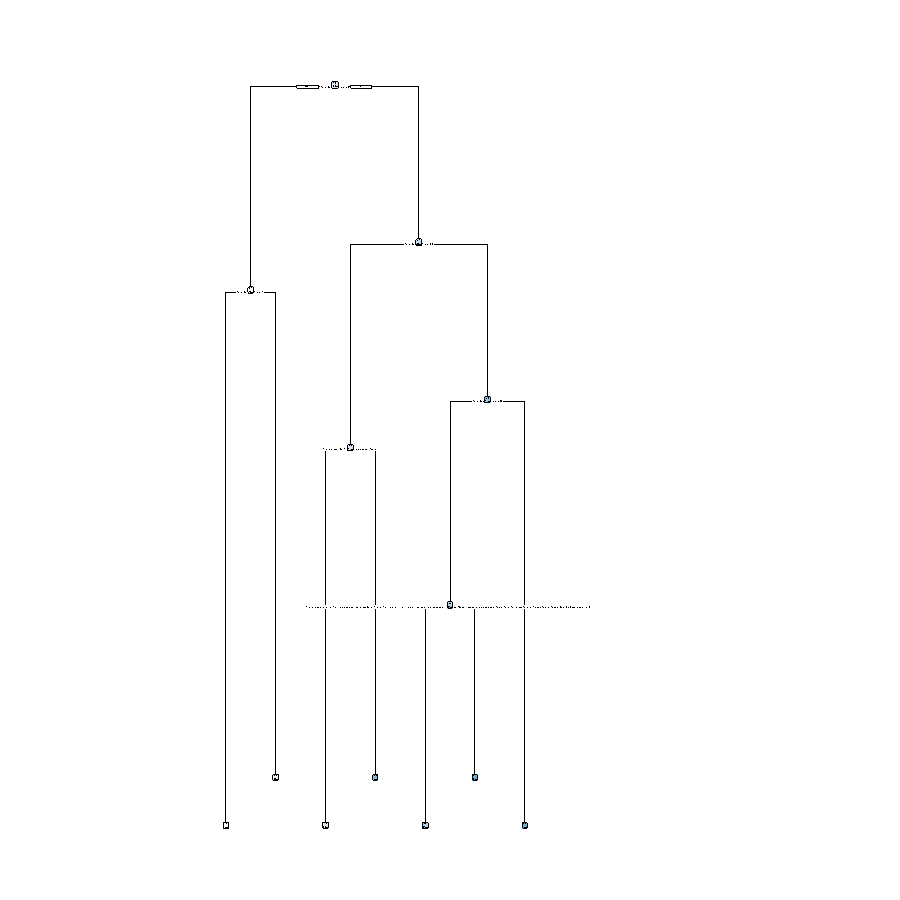
\includegraphics[width=.6\linewidth]{figure/Task2-Rnwauto-report-1} 

}


\begin{kframe}\begin{alltt}
\hlstd{default.model} \hlkwb{<-} \hlkwd{rpart}\hlstd{(Hidden.Gem.Score}\hlopt{~}\hlstd{Languages}\hlopt{+}\hlstd{Runtime}\hlopt{+}\hlstd{IMDb.Score}\hlopt{+}\hlstd{Rotten.Tomatoes.Score}\hlopt{+}\hlstd{Metacritic.Score,} \hlkwc{data} \hlstd{= train)}
\hlstd{info.model} \hlkwb{<-} \hlkwd{rpart}\hlstd{(Hidden.Gem.Score}\hlopt{~}\hlstd{Languages}\hlopt{+}\hlstd{Runtime}\hlopt{+}\hlstd{IMDb.Score}\hlopt{+}\hlstd{Rotten.Tomatoes.Score}\hlopt{+}\hlstd{Metacritic.Score,} \hlkwc{data} \hlstd{= train,} \hlkwc{parms}\hlstd{=}\hlkwd{list}\hlstd{(}\hlkwc{split}\hlstd{=}\hlstr{"information"}\hlstd{))}
\hlstd{overfit.model} \hlkwb{<-} \hlkwd{rpart}\hlstd{(Hidden.Gem.Score}\hlopt{~}\hlstd{Languages}\hlopt{+}\hlstd{Runtime}\hlopt{+}\hlstd{IMDb.Score}\hlopt{+}\hlstd{Rotten.Tomatoes.Score}\hlopt{+}\hlstd{Metacritic.Score,} \hlkwc{data} \hlstd{= train,}\hlkwc{maxdepth}\hlstd{=} \hlnum{5}\hlstd{,} \hlkwc{minsplit}\hlstd{=}\hlnum{2}\hlstd{,}\hlkwc{minbucket} \hlstd{=} \hlnum{1}\hlstd{)}
\hlstd{one.rule.model}\hlkwb{<-} \hlkwd{rpart}\hlstd{(Hidden.Gem.Score}\hlopt{~}\hlstd{Languages}\hlopt{+}\hlstd{Runtime}\hlopt{+}\hlstd{IMDb.Score}\hlopt{+}\hlstd{Rotten.Tomatoes.Score}\hlopt{+}\hlstd{Metacritic.Score,} \hlkwc{data} \hlstd{= train,} \hlkwc{maxdepth} \hlstd{=}\hlnum{1}\hlstd{)}
\hlkwd{rpart.plot}\hlstd{(one.rule.model,} \hlkwc{main}\hlstd{=}\hlstr{"Single Rule Model"}\hlstd{)}
\end{alltt}
\end{kframe}

{\centering 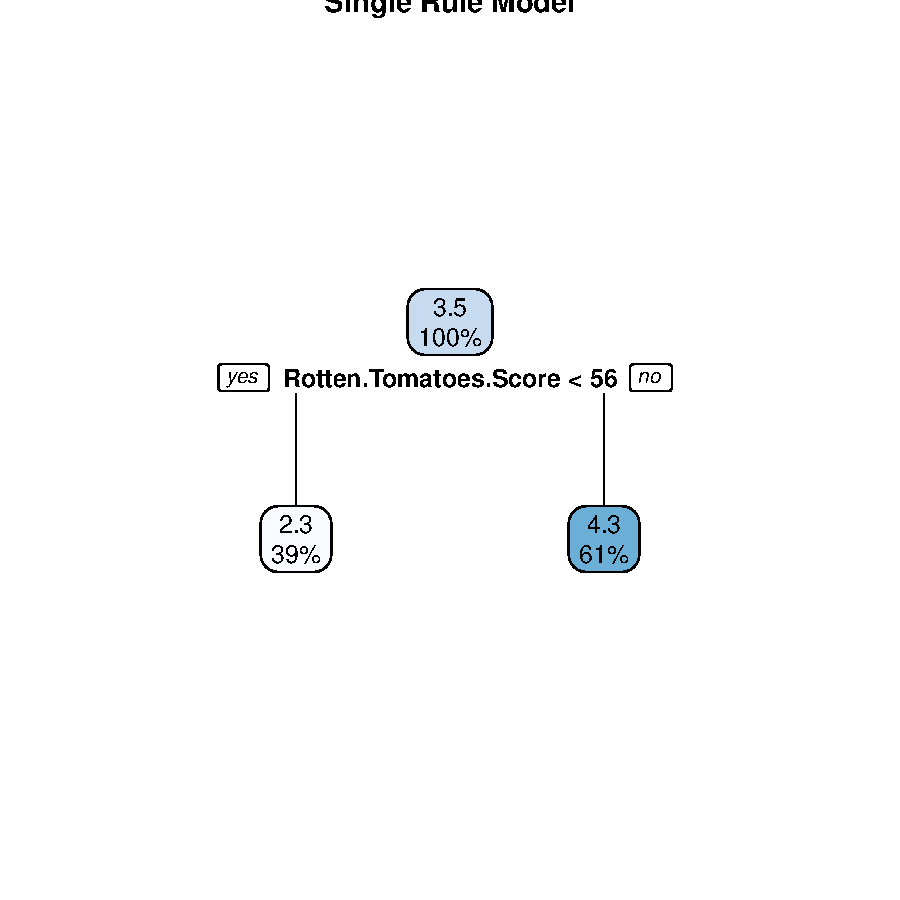
\includegraphics[width=.6\linewidth]{figure/Task2-Rnwauto-report-2} 

}


\begin{kframe}\begin{alltt}
\hlstd{super.overfit.model} \hlkwb{<-} \hlkwd{rpart}\hlstd{(Hidden.Gem.Score}\hlopt{~}\hlstd{Languages}\hlopt{+}\hlstd{Runtime}\hlopt{+}\hlstd{IMDb.Score}\hlopt{+}\hlstd{Rotten.Tomatoes.Score}\hlopt{+}\hlstd{Metacritic.Score,} \hlkwc{data} \hlstd{= train,} \hlkwc{minsplit}\hlstd{=}\hlnum{2}\hlstd{,}\hlkwc{minbucket} \hlstd{=} \hlnum{1}\hlstd{,} \hlkwc{cp} \hlstd{=} \hlnum{0.0001}\hlstd{)}
\hlkwd{rpart.plot}\hlstd{(super.overfit.model,} \hlkwc{main} \hlstd{=} \hlstr{"Really Overfit"}\hlstd{)}
\end{alltt}


{\ttfamily\noindent\color{warningcolor}{\#\# Warning: labs do not fit even at cex 0.15, there may be some overplotting}}\end{kframe}

{\centering 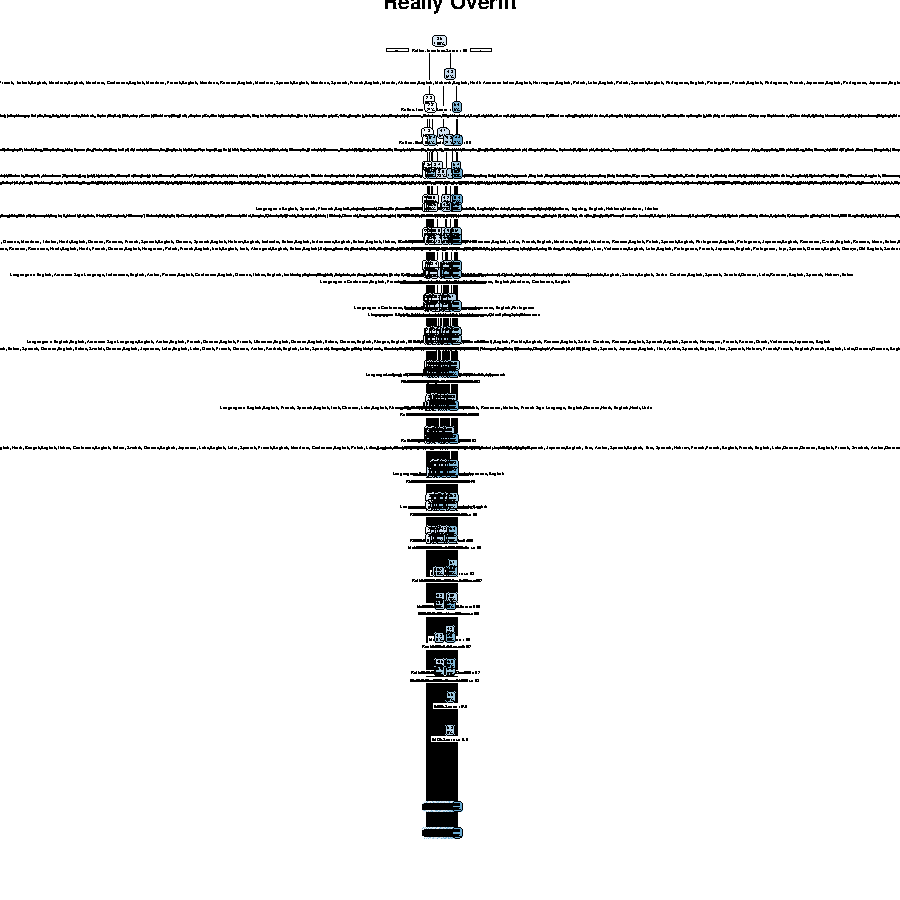
\includegraphics[width=.6\linewidth]{figure/Task2-Rnwauto-report-3} 

}


\begin{kframe}\begin{alltt}
\hlstd{cost.driven.model} \hlkwb{<-} \hlkwd{rpart}\hlstd{(Hidden.Gem.Score}\hlopt{~}\hlstd{Languages}\hlopt{+}\hlstd{Runtime}\hlopt{+}\hlstd{IMDb.Score}\hlopt{+}\hlstd{Rotten.Tomatoes.Score}\hlopt{+}\hlstd{Metacritic.Score,}\hlkwc{data}\hlstd{=train,}\hlkwc{parms}\hlstd{=}\hlkwd{list}\hlstd{(}\hlkwc{loss}\hlstd{=}\hlkwd{matrix}\hlstd{(}\hlkwd{c}\hlstd{(}\hlnum{0}\hlstd{,}\hlnum{1}\hlstd{,}\hlnum{5}\hlstd{,}\hlnum{0}\hlstd{),}\hlkwc{byrow}\hlstd{=}\hlnum{TRUE}\hlstd{,}\hlkwc{nrow}\hlstd{=}\hlnum{2}\hlstd{)))}
\end{alltt}
\end{kframe}
\end{knitrout}

The R session information (including the OS info, R version and all
packages used):

\begin{knitrout}
\definecolor{shadecolor}{rgb}{0.969, 0.969, 0.969}\color{fgcolor}\begin{kframe}
\begin{alltt}
\hlkwd{sessionInfo}\hlstd{()}
\end{alltt}
\begin{verbatim}
## R version 4.1.1 (2021-08-10)
## Platform: x86_64-w64-mingw32/x64 (64-bit)
## Running under: Windows 10 x64 (build 19044)
## 
## Matrix products: default
## 
## locale:
## [1] LC_COLLATE=English_Canada.1252  LC_CTYPE=English_Canada.1252   
## [3] LC_MONETARY=English_Canada.1252 LC_NUMERIC=C                   
## [5] LC_TIME=English_Canada.1252    
## 
## attached base packages:
## [1] stats     graphics  grDevices utils     datasets  methods   base     
## 
## other attached packages:
##  [1] RColorBrewer_1.1-2 rattle_5.4.0       bitops_1.0-7       rpart.plot_3.1.0  
##  [5] rpart_4.1-15       knitr_1.36         ggpubr_0.4.0       forcats_0.5.1     
##  [9] stringr_1.4.0      dplyr_1.0.7        purrr_0.3.4        readr_2.0.2       
## [13] tidyr_1.1.4        tibble_3.1.5       ggplot2_3.3.5      tidyverse_1.3.1   
## [17] here_1.0.1        
## 
## loaded via a namespace (and not attached):
##  [1] Rcpp_1.0.7       lubridate_1.8.0  assertthat_0.2.1 rprojroot_2.0.2  utf8_1.2.2      
##  [6] R6_2.5.1         cellranger_1.1.0 backports_1.2.1  reprex_2.0.1     evaluate_0.14   
## [11] httr_1.4.2       highr_0.9        pillar_1.6.4     rlang_0.4.11     readxl_1.3.1    
## [16] rstudioapi_0.13  car_3.0-12       tinytex_0.34     munsell_0.5.0    broom_0.7.9     
## [21] compiler_4.1.1   modelr_0.1.8     xfun_0.26        pkgconfig_2.0.3  tidyselect_1.1.1
## [26] fansi_0.5.0      crayon_1.4.1     tzdb_0.1.2       dbplyr_2.1.1     withr_2.4.2     
## [31] grid_4.1.1       jsonlite_1.7.2   gtable_0.3.0     lifecycle_1.0.1  DBI_1.1.1       
## [36] magrittr_2.0.1   scales_1.1.1     cli_3.0.1        stringi_1.7.5    carData_3.0-4   
## [41] ggsignif_0.6.3   fs_1.5.0         xml2_1.3.2       ellipsis_0.3.2   generics_0.1.0  
## [46] vctrs_0.3.8      cowplot_1.1.1    tools_4.1.1      glue_1.4.2       hms_1.1.1       
## [51] abind_1.4-5      colorspace_2.0-2 rstatix_0.7.0    rvest_1.0.2      haven_2.4.3
\end{verbatim}
\begin{alltt}
\hlkwd{Sys.time}\hlstd{()}
\end{alltt}
\begin{verbatim}
## [1] "2021-12-23 21:26:58 EST"
\end{verbatim}
\end{kframe}
\end{knitrout}


\end{document}
